% ==========================================================================================================================
\section{Modelo de administración de red de SNMP}
% ==========================================================================================================================

\noindent
A continuación se muestran se muestran los resultados de la herramienta creada por medio de las siguientes operaciones.

\noindent
\newline
\textbf{Operación 1:} Se agrega un agente LINUX con el nombre ''comunidadEquipo3grupo4CM1''. Haciendo una consulta SNMP con la comunidad dada de alta obtenemos la información de ésta misma, como se muestra en la imagen debajo.  
 
\begin{figure}[htbp!]
	\centering
		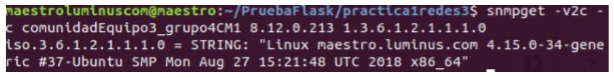
\includegraphics[width=0.8\textwidth]{images/tarea3/op1}
	\caption{Operación 1a.}
\end{figure}

\noindent
Para el agente de Windows, se configuró con el mismo nombre del agente para Linux, la diferencia radica en que la ip de ambos agentes es distinta. En la siguiente figura se puede observar que al hacer la consulta snmp, el resultado arroja información de software “Windows”. 

\begin{figure}[htbp!]
	\centering
		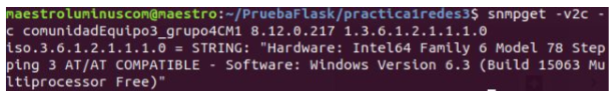
\includegraphics[width=0.8\textwidth]{images/tarea3/op1b}
	\caption{Operación 1b.}
\end{figure}

\noindent
\textbf{Operación 2:} Se agrega el agente windows previamente creado como agente a observium, como se puede ver a continuación.

\begin{figure}[htbp!]
	\centering
		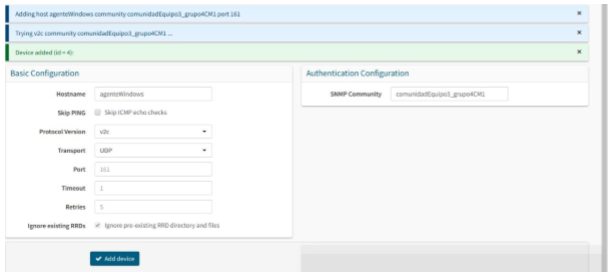
\includegraphics[width=0.8\textwidth]{images/tarea3/op2a}
	\caption{Operación 2a.}
\end{figure}

\begin{figure}[htbp!]
	\centering
		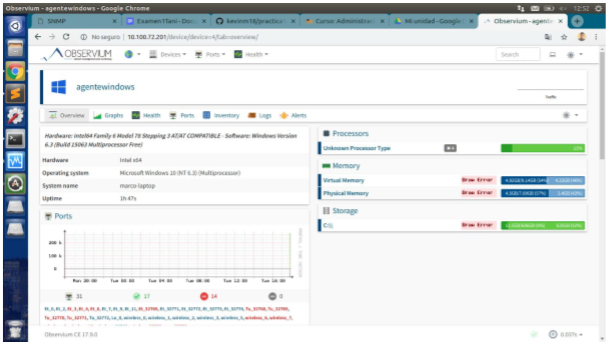
\includegraphics[width=0.8\textwidth]{images/tarea3/op2b}
	\caption{Operación 2b.}
\end{figure}

\begin{figure}[htbp!]
	\centering
		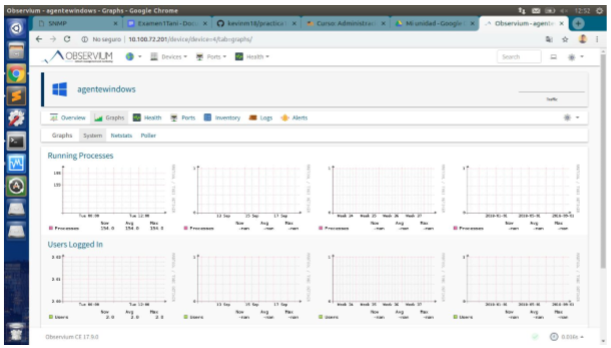
\includegraphics[width=0.8\textwidth]{images/tarea3/op2c}
	\caption{Operación 2c.}
\end{figure}

\pagebreak
\noindent
\textbf{Operación 3:} Se agrega un nuevo agente usando nuestra herramienta creada, para ello se requieren los siguientes datos del agente: Nombre (UbuntuExamenEquipo3), host (8.12.0.123), comunidad (comunidadEquipo3grupo4CM1), version SNMP (v2) y puerto (8012), al presionar el botón “agregar agente”. 

\begin{figure}[htbp!]
	\centering
		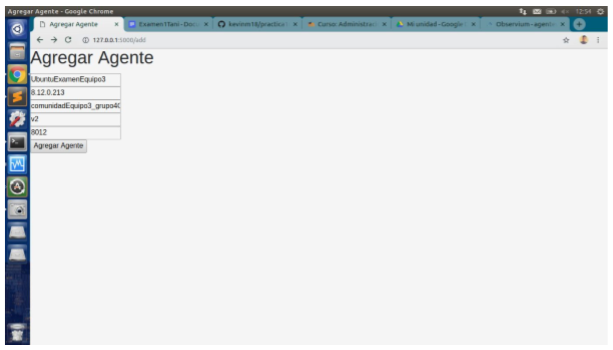
\includegraphics[width=0.8\textwidth]{images/tarea3/op3a}
	\caption{Operación 3c.}
\end{figure}

\noindent 
Como se puede ver en la lista de agentes agregados, se muestra el agente recién añadido en el último renglón, con los datos arriba descritos, mostrando que el agente se añadió correctamente. Asimismo, se muestra el estado de las interfaces del agente agregado.  

\begin{figure}[htbp!]
	\centering
		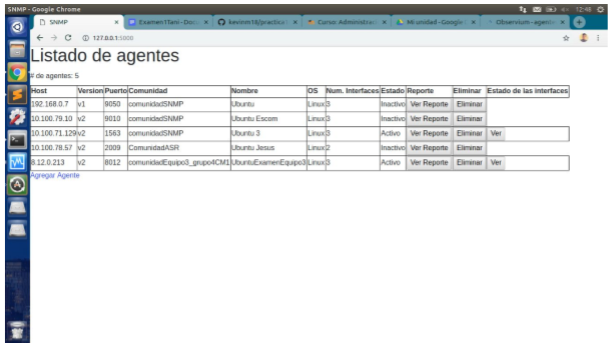
\includegraphics[width=0.8\textwidth]{images/tarea3/op3b}
	\caption{Operación 3b.}
\end{figure}

\begin{figure}[htbp!]
	\centering
		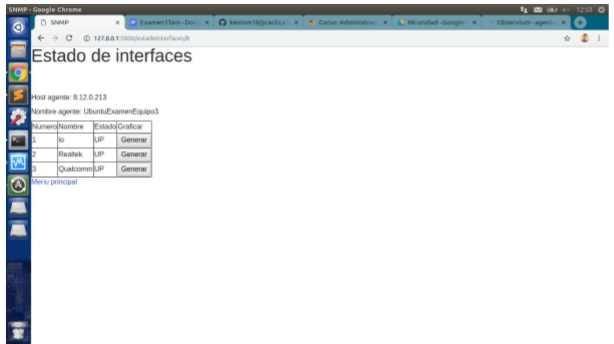
\includegraphics[width=0.8\textwidth]{images/tarea3/op3c}
	\caption{Operación 3c.}
\end{figure}

\noindent
Finalmente, aquí se muestran las funciones (de nuestra herramienta) que hacen posible agregar nuevos agentes. Primeramente tenemos la función “agregar” que realiza consultas SNMP para comprobar que los datos introducidos sean correctos, de ser esto cierto y al lograr exitosamente las consultas SNMP, se inserta el agente, por medio de la función “insertar”, ambas funciones se muestran en las imágenes debajo.

\begin{figure}[htbp!]
	\centering
		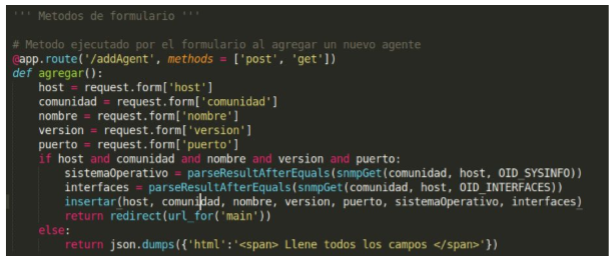
\includegraphics[width=0.8\textwidth]{images/tarea3/op3d}
	\caption{Operación 3d.}
\end{figure}

\begin{figure}[htbp!]
	\centering
		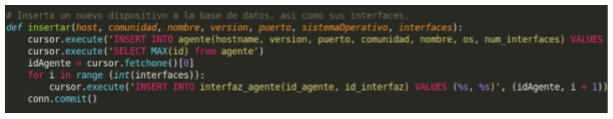
\includegraphics[width=0.8\textwidth]{images/tarea3/op3e}
	\caption{Operación 3e.}
\end{figure}

\noindent
También se agregan 5 consultas SNMP sobre objetos de la MIB. Las imágenes debajo muestran las gráficas de cada una, mostrando además el nombre de la variable analizada debajo de la gráfica. Dichas gráficas se genera con la herramienta realizada.  
 
\begin{figure}[htbp!]
	\centering
		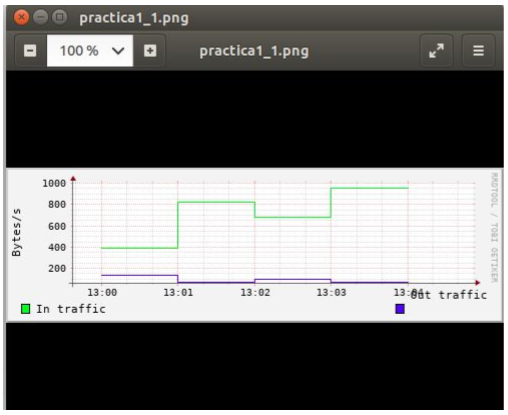
\includegraphics[width=0.8\textwidth]{images/tarea3/op3f}
	\caption{Operación 3f.}
\end{figure}

\begin{figure}[htbp!]
	\centering
		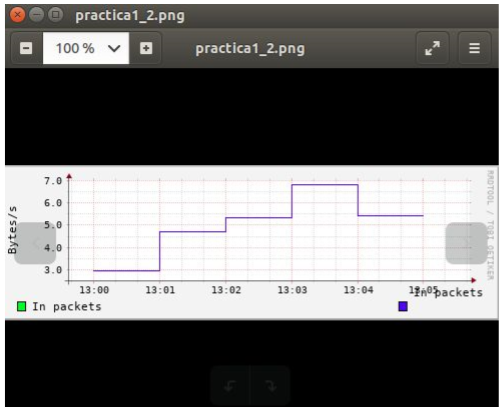
\includegraphics[width=0.8\textwidth]{images/tarea3/op3g}
	\caption{Operación 3g.}
\end{figure}

\begin{figure}[htbp!]
	\centering
		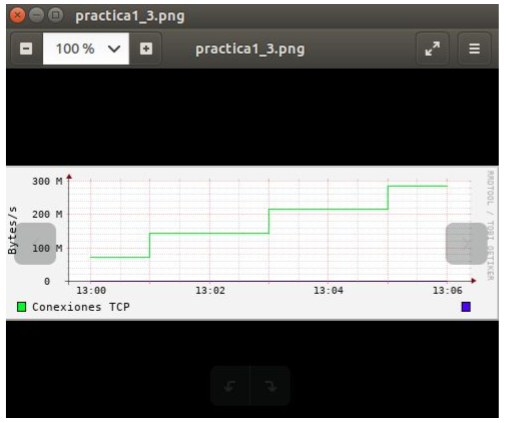
\includegraphics[width=0.8\textwidth]{images/tarea3/op3h}
	\caption{Operación 3h.}
\end{figure}

\begin{figure}[htbp!]
	\centering
		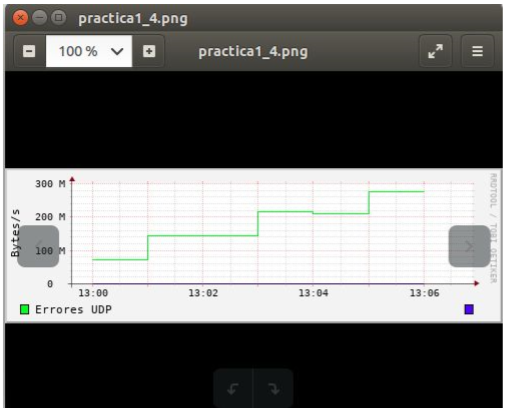
\includegraphics[width=0.8\textwidth]{images/tarea3/op3i}
	\caption{Operación 3i.}
\end{figure}

\begin{figure}[htbp!]
	\centering
		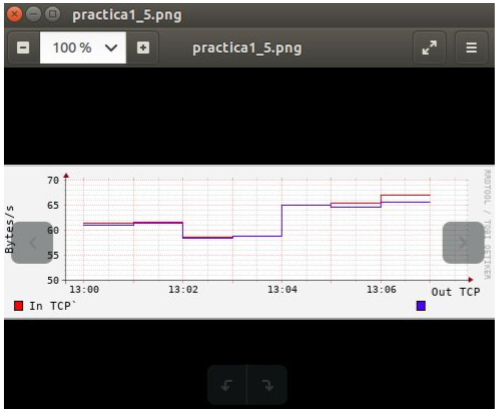
\includegraphics[width=0.8\textwidth]{images/tarea3/op3j}
	\caption{Operación 3j.}
\end{figure}

\noindent
\textbf{Operación 4:} Se agrega agente3 de la maestra. 

\begin{figure}[htbp!]
	\centering
		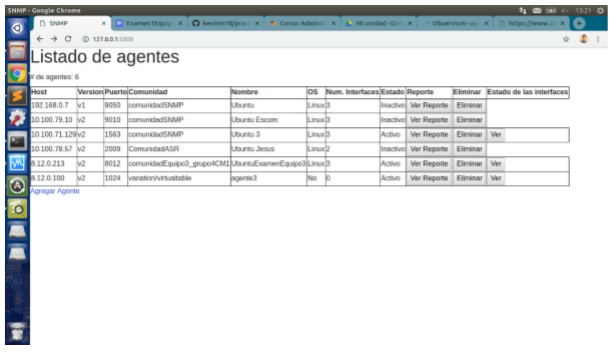
\includegraphics[width=0.8\textwidth]{images/tarea3/op4a}
	\caption{Operación 4a.}
\end{figure}

\noindent
Se muestra el OID que construimos para nuestro apartado (apartado 3 del la tabla escrita en el examen en el problema 4), ifInUcastPkts 

\begin{figure}[htbp!]
	\centering
		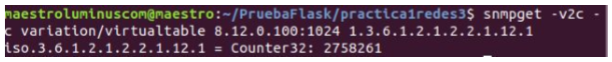
\includegraphics[width=0.8\textwidth]{images/tarea3/op4b}
	\caption{Operación 4b.}
\end{figure}

\noindent
Aquí se muestra la imagen de lo antes analiszado.  

\begin{figure}[htbp!]
	\centering
		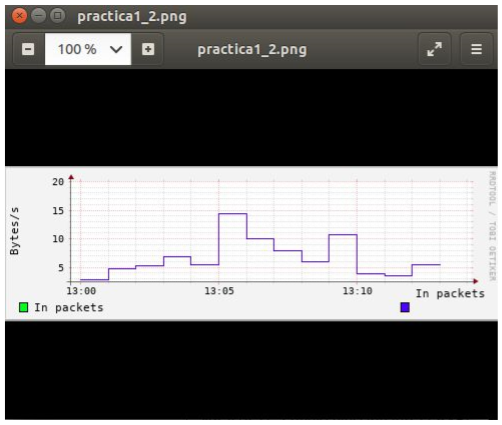
\includegraphics[width=0.8\textwidth]{images/tarea3/op4c}
	\caption{Operación 4c.}
\end{figure}

\noindent
Debajo se muestra el código de muestra que todo se hace de manera concurrente.  

\begin{figure}[htbp!]
	\centering
		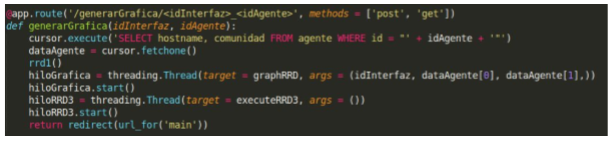
\includegraphics[width=0.8\textwidth]{images/tarea3/op4d}
	\caption{Operación 4d.}
\end{figure}

\noindent
\textbf{Operación 5:} Debajo se muestra el nodo antes de la información  

\begin{figure}[htbp!]
	\centering
		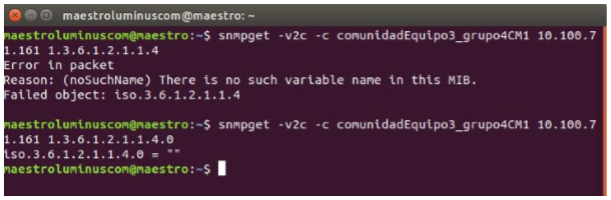
\includegraphics[width=0.8\textwidth]{images/tarea3/op5}
	\caption{Operación 5.}
\end{figure}